\documentclass[../LuanVan.tex]{subfiles}
\begin{document}

%------------------------------------------------------------------
\section{Môi trường và công cụ triển khai}
\label{sec:moitruong}
%------------------------------------------------------------------

\subsection{Bối cảnh chuẩn hóa NIST FIPS 203 và yêu cầu nền tảng}

Trong đặc tả chính thức của Viện Tiêu chuẩn và Công nghệ Quốc gia Hoa Kỳ (NIST FIPS 203, phát hành tháng 8/2024)~\cite{FIPS203}, thuật toán CRYSTALS-Kyber đã được chuẩn hóa với tên gọi chính thức là ML-KEM (Module-Lattice-Based Key-Encapsulation Mechanism). Theo đặc tả tiêu chuẩn này:
\begin{itemize}[leftmargin=2cm]
    \item \textbf{Bắt buộc sử dụng NTT}: Phép nhân đa thức trên vành $\mathcal{R}_q = \mathbb{Z}_q[X]/(X^n+1)$ (với tham số $n=256, q=3329$) bắt buộc phải được chuyển đổi sang miền NTT (Number Theoretic Transform). Kỹ thuật này giảm độ phức tạp tính toán từ nhân chập đa thức truyền thống $\mathcal{O}(n^2)$ xuống còn $\mathcal{O}(n \log n)$.
    \item \textbf{Tối ưu hóa sâu theo chuẩn}: Trong các thư viện sản xuất thực tế (như OpenSSL, BoringSSL, liboqs), khóa công khai và các ma trận đa thức $\mathbf{A}$ được lưu trữ và thao tác trực tiếp trong miền NTT để hạn chế tối đa chi phí chuyển đổi thuận/nghịch.
    \item \textbf{Loại bỏ nhân đa thức truyền thống}: Phép nhân đa thức thông thường hầu như không bao giờ được sử dụng trong triển khai thực tế vì tốc độ rất chậm và tạo điểm nghẽn hiệu năng nghiêm trọng; nó chỉ tồn tại ở các tài liệu lý thuyết nhập môn hoặc các bản mẫu thử nghiệm tối giản.
\end{itemize}

Do đó, toàn bộ hệ thống KyberGuard trong nghiên cứu này tuân thủ hoàn toàn chuẩn FIPS 203, sử dụng biến đổi NTT cho toàn bộ các phép tính đại số trên vành đa thức. Mục tiêu cốt lõi của đề tài tập trung vào bài toán: Đánh giá và nâng cao an toàn kênh bên thông qua kỹ thuật che mặt nạ ngẫu nhiên $\mathbf{r}$ so với bản gốc chuẩn chưa che mặt nạ.

\subsection{Ngôn ngữ lập trình và các thư viện phụ thuộc}

Hệ thống được phát triển và thực nghiệm trên môi trường ngôn ngữ Python phiên bản 3.12.10 (kiến trúc 64-bit), cung cấp khả năng kiểm chứng thuật toán rõ ràng và minh bạch. Bảng~\ref{tab:dependencies} liệt kê các thư viện phụ thuộc chính.

\begin{table}[H]
\centering
\caption{Danh sách thư viện và vai trò trong hệ thống (thực tế triển khai)}
\label{tab:dependencies}
\begin{tabularx}{\textwidth}{l l X}
\toprule
\textbf{Thư viện} & \textbf{Phiên bản} & \textbf{Vai trò} \\
\midrule
\texttt{numpy} & 1.26.1 & Thao tác cấu trúc mảng và vector hệ số đa thức \\
\texttt{pycryptodome} & 3.19.0 & Các hàm băm SHA3-256, SHA3-512, SHAKE-128, SHAKE-256 chuẩn FIPS 202 \\
\texttt{secrets} & (built-in) & Bộ sinh số ngẫu nhiên an toàn (CSPRNG) cấp hệ điều hành phục vụ tạo mặt nạ $\mathbf{r}$ \\
\texttt{matplotlib} & 3.8.2 & Vẽ biểu đồ phân tán tương quan (Scatter Plot) đánh giá kênh bên \\
\texttt{pytest} & 7.4.3 & Framework kiểm thử đơn vị tự động \\
\texttt{invoke} & 2.2.0 & Tự động hóa tác vụ phát triển (test, benchmark, lint) \\
\bottomrule
\end{tabularx}
\end{table}

\subsection{Môi trường thực thi}

Các thử nghiệm đánh giá hiệu năng và mô phỏng tấn công kênh bên được tiến hành trên thiết bị thực tế có thông số kỹ thuật chi tiết như Bảng~\ref{tab:environment}.

\begin{table}[H]
\centering
\caption{Cấu hình môi trường thực nghiệm thực tế}
\label{tab:environment}
\begin{tabular}{l Y{0.85}}
\toprule
\textbf{Thành phần} & \textbf{Chi tiết cấu hình thực tế} \\
\midrule
Hệ điều hành & Microsoft Windows 11 (kiến trúc 64-bit) \\
Python Runtime & CPython 3.12.10 64-bit (quản lý bởi Poetry) \\
CPU & Intel64 Family 6 Model 140 Stepping 1, GenuineIntel \\
RAM & 16 GB \\
\bottomrule
\end{tabular}
\end{table}

%------------------------------------------------------------------
\section{Triển khai các thành phần của KyberGuard}
\label{sec:trienkhai}
%------------------------------------------------------------------

\subsection{Kiến trúc tổng quan}

Toàn bộ hệ thống được module hóa chặt chẽ. Cấu trúc phân cấp các thư mục và tệp mã nguồn trong dự án được tổ chức trực quan như Liệt kê~\ref{lst:dirtree}.

\begin{lstlisting}[style=treestyle, caption={Cấu trúc mã nguồn dự án KyberGuard}, label={lst:dirtree}]
kyber/
├── kyber/                          # Package chinh cua he thong KyberGuard
│   ├── constants.py                # Tham so Kyber1024 theo FIPS 203 (q=3329, n=256, k=4)
│   ├── ccakem.py                   # IND-CCA2 KEM (Bien doi Fujisaki-Okamoto)
│   ├── side_channel_poc.py         # Mo phong tan cong kenh ben (Timing & DPA)
│   ├── encryption/                 # CPAPKE: ma hoa va giai ma khoa cong khai
│   │   ├── keygen.py               # Sinh cap khoa CPAPKE
│   │   ├── encrypt.py              # Ma hoa CPAPKE
│   │   ├── decrypt.py              # Giai ma chuan FIPS 203 (Ban goc, chua bao ve)
│   │   └── decrypt_blinded.py      # Giai ma co mat na r (Ban bao ve kenh ben)
│   ├── entities/
│   │   └── polring.py              # Cau truc du lieu vanh da thuc PolynomialRing
│   └── utils/                      # Cac ham toan hoc va thuat toan bo tro
│       ├── ntt.py                  # Bien doi so hoc NTT (Cooley-Tukey, base-mul)
│       ├── byte_conversion.py      # Chuyen doi byte <-> integer <-> bit array
│       ├── cbd.py                  # Centered Binomial Distribution sampling
│       ├── compression.py          # Nen/giai nen he so da thuc modulo q
│       ├── encoding.py             # Ma hoa/giai ma da thuc <-> byte array
│       ├── parse.py                # Rejection sampling tu XOF sang da thuc
│       ├── pseudo_random.py        # Cac ham bam SHA-3 (H, G, KDF, XOF, PRF)
│       └── round.py                # Ham lam tron chuan (half-up rounding)
├── tests/                          # 70 unit tests kiem thu tinh dung dan (pytest)
├── perf_tests/                     # Benchmark hieu nang KEM va tich hop AES-GCM
├── docs/                           # Tai lieu thiet ke va dac ta ky thuat
├── images/                         # Do thi phan tan (scatter plots) cho bao cao
├── demo_comparison.py              # So sanh & benchmark Ban goc vs Ban co mat na r
├── test_dpa_quick.py               # Script kiem tra nhanh tuong quan DPA
├── export_figures.py               # Tu dong xuat bieu do cho bao cao LaTeX
└── pyproject.toml                  # Quan ly cau hinh du an va dependencies (Poetry)
\end{lstlisting}

Bảng~\ref{tab:modules} tóm tắt chi tiết vai trò của các tệp mã nguồn và module cốt lõi trong hệ sinh thái KyberGuard.

\begin{table}[H]
\centering
\caption{Các module chính của hệ thống}
\label{tab:modules}
\begin{tabular}{L{3cm} Y{0.3} Y{0.5}}
\toprule
\textbf{Thành phần} & \textbf{Tệp mã nguồn} & \textbf{Chức năng} \\
\midrule
Tham số chuẩn & \path{constants.py} & Tham số Kyber1024 theo FIPS 203: $n=256, q=3329, k=4$ \\
Vành đa thức & \path{entities/polring.py} & Lớp \texttt{PolynomialRing} biểu diễn phần tử trên $\mathcal{R}_q$ \\
Biến đổi số học & \path{utils/ntt.py} & Biến đổi NTT, INTT và phép nhân cơ sở (base-mul) \\
Sinh khóa & \path{encryption/keygen.py} & Sinh cặp khóa công khai / bí mật CPAPKE \\
Mã hóa & \path{encryption/encrypt.py} & Thuật toán đóng gói bản mã CPAPKE \\
Giải mã gốc & \path{encryption/decrypt.py} & Giải mã chuẩn FIPS 203 (bản gốc, chưa bảo vệ mặt nạ) \\
Giải mã có mặt nạ & \path{encryption/decrypt_blinded.py} & Giải mã cải tiến có mặt nạ $\mathbf{r}$ (bảo vệ chống kênh bên) \\
Cơ chế KEM & \path{ccakem.py} & Biến đổi Fujisaki-Okamoto đạt an toàn IND-CCA2 \\
Hàm giả ngẫu nhiên & \path{utils/pseudo_random.py} & Bộ hàm băm SHA-3 và hàm mở rộng SHAKE \\
Đánh giá an toàn & \path{side_channel_poc.py} & Mô phỏng tấn công thời gian (Timing) và năng lượng (DPA) \\
\bottomrule
\end{tabular}
\end{table}

\subsection{Tham số chuẩn Kyber1024 (ML-KEM-1024)}

Hệ thống hiện thực hóa mức bảo mật cao nhất của Kyber -- mức NIST Level 5 (tương đương độ an toàn phá mã của AES-256):

\begin{table}[H]
\centering
\caption{Tham số cấu hình Kyber1024 chuẩn FIPS 203}
\label{tab:kyber_params}
\begin{tabular}{c c l}
\toprule
\textbf{Tham số} & \textbf{Giá trị} & \textbf{Ý nghĩa} \\
\midrule
$n$ & 256 & Bậc của đa thức trên vành $\mathcal{R}_q = \mathbb{Z}_q[X]/(X^{256}+1)$ \\
$q$ & 3329 & Số nguyên tố modulus \\
$k$ & 4 & Kích thước vector/ma trận đa thức \\
$\eta_1, \eta_2$ & 2, 2 & Tham số biên độ phân phối nhị thức tâm \\
$d_u, d_v$ & 11, 5 & Số bit nén cho vector bản mã $\mathbf{u}$ và đa thức $v$ \\
\bottomrule
\end{tabular}
\end{table}

Kích thước khóa và bản mã tương ứng:
\begin{itemize}[leftmargin=2cm]
    \item Khóa bí mật CPAPKE ($sk$): $12 \times k \times n / 8 = 1536$ bytes.
    \item Khóa công khai ($pk$): $12 \times k \times n / 8 + 32 = 1568$ bytes.
    \item Khóa bí mật CCA-KEM: $24 \times k \times n / 8 + 96 = 3168$ bytes.
    \item Bản mã đóng gói ($c$): $d_u \cdot k \cdot n / 8 + d_v \cdot n / 8 = 1568$ bytes.
\end{itemize}

\subsection{Cơ chế biến đổi số học NTT chuẩn hóa}

Đặc tả FIPS 203~\cite{FIPS203} xác định đa thức rút gọn $X^{256} + 1$ phân tích thành 128 nhân tử bậc 2 trên $\mathbb{Z}_q$:
\begin{equation}
X^{256} + 1 \equiv \prod_{i=0}^{127} \bigl(X^2 - \zeta^{2\cdot \text{bitrev}_7(i)+1}\bigr) \pmod q
\end{equation}
với $\zeta = 17$ là căn nguyên thủy bậc 256 của đơn vị trong $\mathbb{Z}_q$ ($17^{128} \equiv -1 \pmod{3329}$).

Mỗi phép nhân hai đa thức trong miền biến đổi bao gồm 128 phép nhân cơ sở (base multiplication) trên vành thương $\mathbb{Z}_q[X]/(X^2 - \zeta_i)$:
\begin{equation}
(a_0 + a_1 X)(b_0 + b_1 X) \bmod (X^2 - \zeta_i) = \underbrace{(a_0 b_0 + a_1 b_1 \zeta_i)}_{c_0} + \underbrace{(a_0 b_1 + a_1 b_0)}_{c_1} X
\end{equation}
Tất cả các phép tính vector ma trận $\mathbf{s}^\top \mathbf{u}$ ở bước giải mã đều được thực hiện qua tích vô hướng trực tiếp trong miền NTT với độ phức tạp $\mathcal{O}(k \cdot n)$.

\subsection{Giải mã bản gốc -- \texttt{decrypt.py}}

Hàm giải mã bản gốc \texttt{decrypt(sk, c)} thực hiện quy trình giải mã chuẩn của Kyber theo FIPS 203:
\begin{enumerate}[leftmargin=2cm]
    \item Giải nén và chuyển vector khóa bí mật $\mathbf{s}$ và bản mã $\mathbf{u}$ sang miền biến đổi: $\hat{\mathbf{s}} = \text{NTT}(\mathbf{s})$, $\hat{\mathbf{u}} = \text{NTT}(\mathbf{u})$.
    \item Tính tích vô hướng: $\hat{\mathbf{w}} = \hat{\mathbf{s}}^\top \odot \hat{\mathbf{u}}$.
    \item Chuyển ngược về miền đa thức: $\mathbf{w} = \text{INTT}(\hat{\mathbf{w}})$.
    \item Phục hồi bản rõ: $m = \text{Encode}\bigl(\text{Compress}(v - \mathbf{w}, 1), 1\bigr)$.
\end{enumerate}

\begin{lstlisting}[language=Python, style=pystyle, caption={Hàm giải mã bản gốc chuẩn hóa -- decrypt() trong decrypt.py}]
def decrypt(private_key: bytes, ciphertext: bytes) -> bytes:
    s_pols = decode(private_key, 12)
    u_bytes = ciphertext[: du * k * n // 8]
    v_bytes = ciphertext[du * k * n // 8 :]

    u_pols = [decompress(pol, du) for pol in decode(u_bytes, du)]
    v_pol  = decompress(decode(v_bytes, dv)[0], dv)

    s_hat = [ntt(polring_to_list(p)) for p in s_pols]
    u_hat = [ntt(polring_to_list(p)) for p in u_pols]
    v_coefs = polring_to_list(v_pol)

    # Tich vo huong truc tiep trong mien bien doi
    s_u_hat = dot_product_ntt(s_hat, u_hat)
    s_dot_u = intt(s_u_hat)

    m_coefs = [(v_coefs[j] - s_dot_u[j]) % q for j in range(n)]
    m_pol = PolynomialRing(m_coefs, check_limits=True)
    return encode(compress([m_pol], 1), 1)
\end{lstlisting}

\subsection{Giải mã cải tiến với mặt nạ ngẫu nhiên \texorpdfstring{$\mathbf{r}$}{r} -- \texttt{decrypt\_blinded.py}}
\label{subsec:blinding}

Trong bản gốc, khóa bí mật $\hat{\mathbf{s}}$ được nhân trực tiếp với bản mã $\hat{\mathbf{u}}$. Điều này tạo ra tương quan công suất tiêu thụ rất mạnh phụ thuộc vào $\hat{\mathbf{s}}$, khiến hệ thống dễ bị tấn công DPA.

\subsubsection{Nguyên lý che mặt nạ}

Để bảo vệ khóa bí mật, kỹ thuật che mặt nạ (Masking / Blinding) được đề xuất:
\begin{enumerate}[leftmargin=2cm]
    \item Sinh vector mặt nạ ngẫu nhiên $\hat{\mathbf{r}} \in \mathbb{Z}_q^{k \times n}$ trực tiếp từ bộ sinh ngẫu nhiên an toàn cấp hệ điều hành (CSPRNG via \texttt{secrets}).
    \item Che giấu khóa bí mật: $\hat{\mathbf{s}}^* = \hat{\mathbf{s}} + \hat{\mathbf{r}} \pmod q$. Giá trị $\hat{\mathbf{s}}$ không bao giờ xuất hiện đơn lẻ trong bất kỳ phép nhân nào.
    \item Tính toán song song hai tích vô hướng:
    \begin{align}
        \widehat{s^* u} &= (\hat{\mathbf{s}}^*)^\top \odot \hat{\mathbf{u}} = (\hat{\mathbf{s}} + \hat{\mathbf{r}})^\top \odot \hat{\mathbf{u}} \\
        \widehat{ru} &= \hat{\mathbf{r}}^\top \odot \hat{\mathbf{u}}
    \end{align}
    \item Khử mặt nạ đại số (De-blinding):
    \begin{equation}
        \widehat{su} = \widehat{s^* u} - \widehat{ru} = (\hat{\mathbf{s}} + \hat{\mathbf{r}})^\top \odot \hat{\mathbf{u}} - \hat{\mathbf{r}}^\top \odot \hat{\mathbf{u}} = \hat{\mathbf{s}}^\top \odot \hat{\mathbf{u}} \pmod q
    \end{equation}
    \item Biến đổi ngược INTT, khôi phục bản rõ và tiến hành \textbf{xóa an toàn bộ nhớ} (ghi đè 0 lên các biến trung gian $\hat{\mathbf{r}}, \hat{\mathbf{s}}^*, \widehat{s^*u}, \widehat{ru}$) để chống rò rỉ bộ nhớ.
\end{enumerate}

\begin{algorithm}[H]
\caption{Giải mã Kyber với cơ chế che mặt nạ ngẫu nhiên $\mathbf{r}$}
\label{alg:decrypt_blinded}
\begin{algorithmic}[1]
\Require Khóa bí mật $\mathrm{sk}$, bản mã $c$
\Ensure Khóa phiên bản rõ $m \in \{0,1\}^{256}$

\State $\mathbf{s} \gets \mathrm{Decode}(\mathrm{sk}, 12)$
\State $(\mathbf{u}, v) \gets \mathrm{DecompressDecode}(c)$

\State $\hat{\mathbf{s}} \gets [\mathrm{NTT}(s_i)]_{i=0}^{k-1}$
\State $\hat{\mathbf{u}} \gets [\mathrm{NTT}(u_i)]_{i=0}^{k-1}$

\State \textit{// --- Che mặt nạ ngẫu nhiên ---}
\State $\hat{\mathbf{r}} \xleftarrow{\$} \mathrm{CSPRNG}(\mathbb{Z}_q^{k \times n})$
    \Comment{Sinh mặt nạ ngẫu nhiên}
\State $\hat{\mathbf{s}}^{*} \gets \hat{\mathbf{s}} + \hat{\mathbf{r}} \pmod q$
    \Comment{Che giấu khóa bí mật}

\State \textit{// --- Tính tích vô hướng ---}
\State $\widehat{s^{*}u} \gets \mathrm{DotProduct}(\hat{\mathbf{s}}^{*}, \hat{\mathbf{u}})$
\State $\widehat{ru} \gets \mathrm{DotProduct}(\hat{\mathbf{r}}, \hat{\mathbf{u}})$

\State \textit{// --- Khử mặt nạ (de-blinding) ---}
\State $\widehat{su} \gets \widehat{s^{*}u} - \widehat{ru} \pmod q$
    \Comment{Khôi phục $\hat{\mathbf{s}}^{\top} \odot \hat{\mathbf{u}}$}

\State $\mathbf{w} \gets \mathrm{INTT}(\widehat{su})$
\State $m \gets v - \mathbf{w} \pmod q$

\State \textit{// --- Xóa an toàn dữ liệu trung gian ---}
\State $\mathrm{Zeroize}(\hat{\mathbf{r}}, \hat{\mathbf{s}}^{*}, \widehat{s^{*}u}, \widehat{ru}, \widehat{su})$

\State \Return $\mathrm{Encode}(\mathrm{Compress}(m, 1), 1)$
\end{algorithmic}
\end{algorithm}

\begin{lstlisting}[language=Python, style=pystyle, caption={Hàm decrypt\_blinded() trong decrypt\_blinded.py}]
def decrypt_blinded(private_key: bytes, ciphertext: bytes) -> bytes:
    s_pols = decode(private_key, 12)
    u_bytes = ciphertext[: du * k * n // 8]
    v_bytes = ciphertext[du * k * n // 8 :]
    u_pols = [decompress(pol, du) for pol in decode(u_bytes, du)]
    v_pol  = decompress(decode(v_bytes, dv)[0], dv)

    s_hat = [ntt(polring_to_list(p)) for p in s_pols]
    u_hat = [ntt(polring_to_list(p)) for p in u_pols]
    v_coefs = polring_to_list(v_pol)

    # Sinh mat na r truc tiep bang CSPRNG va che giau khoa
    r_hat = _random_ntt_vector(k)
    s_star_hat = [add_ntt(s_hat[i], r_hat[i]) for i in range(k)]

    # Tich vo huong: s khong bao gio xuat hien don le
    s_star_u_hat = dot_product_ntt(s_star_hat, u_hat)
    r_u_hat      = dot_product_ntt(r_hat, u_hat)
    s_u_hat      = sub_ntt(s_star_u_hat, r_u_hat)  # Khu mat na

    s_dot_u = intt(s_u_hat)
    m_coefs = [(v_coefs[j] - s_dot_u[j]) % q for j in range(n)]

    # Xoa sach bo nho dem
    _erase_vector(r_hat); _erase_vector(s_star_hat)
    _erase_list(s_star_u_hat); _erase_list(r_u_hat); _erase_list(s_u_hat)

    return encode(compress([PolynomialRing(m_coefs)], 1), 1)
\end{lstlisting}

%------------------------------------------------------------------
\section{Kiểm thử tính đúng đắn}
\label{sec:kiemthu}
%------------------------------------------------------------------

\subsection{Kiểm thử đơn vị và kiểm thử tích hợp}

Hệ thống được kiểm thử tự động với 70 test case bao phủ toàn bộ các module từ chuyển đổi byte, lấy mẫu CBD, nén hệ số đến tích hợp KEM hoàn chỉnh:

\begin{lstlisting}[language=Python, style=pystyle, caption={Kiểm thử tích hợp KEM chuẩn}]
def test_ccakem_integration(self):
    private_key, public_key = ccakem_generate_keys()
    ciphertext, shared_secret1 = ccakem_encrypt(public_key)
    shared_secret2 = ccakem_decrypt(ciphertext, private_key)
    self.assertEqual(shared_secret1, shared_secret2)
\end{lstlisting}

\subsection{Xác thực tính tương đương đại số khi thêm mặt nạ \texorpdfstring{$\mathbf{r}$}{r}}

Để chứng minh việc thêm mặt nạ $\mathbf{r}$ không làm thay đổi bản rõ đầu ra, hàm \texttt{verify\_correctness()} tiến hành so sánh kết quả giải mã giữa bản gốc và bản có mặt nạ trên hàng loạt cặp khóa ngẫu nhiên:
\begin{equation}
\forall (\text{sk}, c): \quad \texttt{decrypt}(\text{sk}, c) \equiv \texttt{decrypt\_blinded}(\text{sk}, c)
\end{equation}

Đẳng thức đại số đảm bảo tính đúng đắn tuyệt đối:
\begin{equation}
(v + \hat{\mathbf{r}}^\top \mathbf{u}) - (\mathbf{s} + \hat{\mathbf{r}})^\top \mathbf{u} = v - \mathbf{s}^\top \mathbf{u} \pmod q
\end{equation}

% ===== KẾT QUẢ CHẠY THỰC TẾ =====
% TODO: Chèn ảnh chụp kết quả chạy pytest (tất cả test PASS)
% \begin{figure}[H]
%     \centering
%     \includegraphics[width=0.9\textwidth]{images/pytest_results.png}
%     \caption{Kết quả chạy kiểm thử đơn vị bằng pytest -- 100\% test PASS}
%     \label{fig:pytest_results}
% \end{figure}

% TODO: Chèn ảnh chụp kết quả verify correctness
% \begin{figure}[H]
%     \centering
%     \includegraphics[width=0.9\textwidth]{images/verify_correctness.png}
%     \caption{Kết quả xác thực tính đúng đắn: decrypt() $\equiv$ decrypt\_blinded() trên các cặp khóa ngẫu nhiên}
%     \label{fig:verify_correctness}
% \end{figure}

%------------------------------------------------------------------
\section{Phương pháp đánh giá an toàn}
\label{sec:phuongphap}
%------------------------------------------------------------------

Nghiên cứu áp dụng hai phương pháp đánh giá kênh bên thực nghiệm nhằm so sánh định lượng giữa \textbf{Bản gốc} và \textbf{Bản có mặt nạ $\mathbf{r}$}.

\subsection{Phương pháp 1: Đánh giá tấn công thời gian (Timing Attack)}

\begin{itemize}[leftmargin=2cm]
    \item \textbf{Mục tiêu}: Kiểm tra xem thời gian thực thi của thuật toán giải mã có phụ thuộc vào dữ liệu khóa bí mật hay không.
    \item \textbf{Quy trình}: Giải mã $N$ bản mã ngẫu nhiên khác nhau. Mỗi bản mã được đo lường 3 lần và lấy giá trị trung vị (median) bằng hàm \texttt{time.perf_counter\_ns()} để loại bỏ nhiễu của hệ điều hành.
    \item \textbf{Chỉ số đánh giá}:
    \begin{itemize}
        \item Hệ số biến thiên: $\text{CV} = \sigma / \mu \times 100\%$.
        \item Hệ số tương quan Pearson $r(\text{timing}, \text{oracle})$ giữa thời gian chạy và Hamming Weight của dữ liệu nhạy cảm.
        \item Ngưỡng an toàn: $|r| \leq 0.1$ biểu thị thời gian thực thi không phụ thuộc vào khóa.
    \end{itemize}
\end{itemize}

\subsection{Phương pháp 2: Đánh giá phân tích năng lượng vi sai (DPA)}

\begin{itemize}[leftmargin=2cm]
    \item \textbf{Mô hình rò rỉ}: Sử dụng mô hình trọng số Hamming (Hamming Weight - HW), mô hình tiêu chuẩn trong phân tích năng lượng phần cứng:
    \begin{equation}
        P \sim \text{HW}(\text{giá trị trung gian})
    \end{equation}
    \item \textbf{Chiến lược mục tiêu (Target Base-Mul)}: Kẻ tấn công nhắm vào một cặp hệ số cơ sở cụ thể $(s_0, s_1)$ trong phép nhân đa thức:
    \begin{equation}
        \text{oracle}[i] = \text{HW}\bigl(s_0 \cdot u_0^{(i)} + s_1 \cdot u_1^{(i)} \cdot \zeta \bmod q\bigr)
    \end{equation}
    \item \textbf{Dấu vết năng lượng mô phỏng (Power Trace)}:
    \begin{itemize}
        \item \textit{Bản gốc (chưa bảo vệ)}: $\text{trace}_{\text{orig}}[i] = \text{oracle}[i] + \mathcal{N}(0, \sigma^2)$ với nhiễu đo lường nhỏ ($\sim 2\%$).
        \item \textit{Bản có mặt nạ $\mathbf{r}$}: $\text{trace}_{\text{blind}}[i] = \text{HW}\bigl((s_0 + r_0) u_0^{(i)} + (s_1 + r_1) u_1^{(i)} \zeta \bmod q\bigr)$ với $r_0, r_1$ được làm mới ngẫu nhiên tại mỗi phiên giải mã.
    \end{itemize}
    \item \textbf{Tiêu chí đánh giá Pearson $|r|$}:
    \begin{itemize}
        \item $|r| > 0.5$: Tương quan mạnh $\rightarrow$ Tấn công thành công, khóa bí mật bị lộ.
        \item $|r| < 0.1$: Không có tương quan tuyến tính $\rightarrow$ Tấn công bị chặn hoàn toàn, hệ thống an toàn.
    \end{itemize}
\end{itemize}

\begin{table}[H]
\centering
\caption{Tóm tắt hai phiên bản được so sánh trong báo cáo}
\label{tab:two_versions}
\begin{tabularx}{\textwidth}{l l X}
\toprule
\textbf{Phiên bản} & \textbf{Hàm thực thi} & \textbf{Cơ chế bảo vệ kênh bên} \\
\midrule
\textbf{Bản gốc} & \texttt{decrypt()} & Thực thi chuẩn FIPS 203, \textbf{không} có mặt nạ bảo vệ \\
\textbf{Bản có mặt nạ $\mathbf{r}$} & \texttt{decrypt\_blinded()} & Khóa $\mathbf{s}$ được che bằng mặt nạ ngẫu nhiên $\mathbf{r}$ trong suốt quá trình nhân \\
\bottomrule
\end{tabularx}
\end{table}

%------------------------------------------------------------------
\section{Kết quả đánh giá an toàn}
\label{sec:ketqua}
%------------------------------------------------------------------

\subsection{Kết quả kiểm tra tính đúng đắn}

Bảng~\ref{tab:verify} thể hiện kết quả kiểm tra 8 phiên giải mã ngẫu nhiên liên tiếp giữa bản gốc \texttt{decrypt()} và bản có mặt nạ \texttt{decrypt\_blinded()}.

\begin{table}[H]
\centering
\caption{Kết quả kiểm tra tính đúng đắn đại số giữa hai phiên bản}
\label{tab:verify}
\begin{tabular}{c c l}
\toprule
\textbf{Phiên} & \textbf{Kết quả} & \textbf{Khóa phiên khôi phục (24 ký tự hex đầu)} \\
\midrule
1 & PASS & \texttt{ec0dbecdb264e936fe364cdb...} \\
2 & PASS & \texttt{6febd165be0f620f2e849d08...} \\
3 & PASS & \texttt{8f91b257c1334e715b07256c...} \\
4 & PASS & \texttt{6ccc63e321ce5403dfe04f66...} \\
5 & PASS & \texttt{c86b08c774fd9067d9b37555...} \\
6 & PASS & \texttt{e8e61fbe9fd1cb44773b1328...} \\
7 & PASS & \texttt{500ec784392c32151f91e624...} \\
8 & PASS & \texttt{2d57a01b2a5b9d80aaac2d92...} \\
\midrule
\multicolumn{3}{c}{\textbf{Tỷ lệ chính xác: 100\% (TẤT CẢ PASS)}} \\
\bottomrule
\end{tabular}
\end{table}

Kết quả chứng minh thực nghiệm hoàn toàn phù hợp với lý thuyết: cơ chế che mặt nạ bảo toàn nguyên vẹn tính đúng đắn của dữ liệu giải mã.

\subsection{Chi phí tính toán tăng thêm (Overhead)}

Bảng~\ref{tab:benchmark} so sánh thời gian thực thi trung bình giữa Bản gốc và Bản có mặt nạ $\mathbf{r}$ trên mẫu 60 bản mã độc lập.

\begin{table}[H]
\centering
\caption{So sánh thời gian thực thi giữa Bản gốc và Bản có mặt nạ $\mathbf{r}$}
\label{tab:benchmark}
\begin{tabular}{l r r r}
\toprule
\textbf{Chỉ số thống kê} & \textbf{Bản gốc ($\mu$s)} & \textbf{Bản có mặt nạ $\mathbf{r}$ ($\mu$s)} & \textbf{Chênh lệch ($\mu$s)} \\
\midrule
Trung bình (Mean) & 16\,043.6 & 17\,245.1 & +1\,201.5 \\
Độ lệch chuẩn (StdDev) & 2\,323.7 & 3\,295.3 & +971.6 \\
Giá trị nhỏ nhất (Min) & 13\,192.1 & 13\,318.1 & +126.0 \\
Giá trị lớn nhất (Max) & 24\,718.9 & 28\,506.3 & +3\,787.4 \\
\midrule
\multicolumn{3}{l}{\textbf{Chi phí tăng thêm (Overhead của mặt nạ $\mathbf{r}$)}} & \textbf{+7.5\%} \\
\bottomrule
\end{tabular}
\end{table}

Chi phí tăng thêm của kỹ thuật che mặt nạ chỉ là \textbf{+7.5\%}, thấp hơn rất nhiều so với ngưỡng khống chế mục tiêu ($< 20\%$). Nguyên nhân là do:
\begin{itemize}[leftmargin=2cm]
    \item Mặt nạ $\hat{\mathbf{r}}$ được sinh ngẫu nhiên trực tiếp trong miền biến đổi, không tốn chi phí thực hiện biến đổi thuận.
    \item Việc che mặt nạ chỉ bổ sung thêm đúng một phép tích vô hướng vector bậc $k$ ($\mathcal{O}(k \cdot n)$), trong khi các biến đổi NTT/INTT chiếm tỷ trọng thời gian lớn nhất không hề bị tăng thêm.
\end{itemize}

% ===== KẾT QUẢ CHẠY THỰC TẾ =====
% TODO: Chèn ảnh chụp kết quả benchmark (bảng thời gian)
% \begin{figure}[H]
%     \centering
%     \includegraphics[width=0.9\textwidth]{images/benchmark_results.png}
%     \caption{Kết quả benchmark thời gian thực tế: Bản gốc vs Bản có mặt nạ $\mathbf{r}$}
%     \label{fig:benchmark}
% \end{figure}

\subsection{Kết quả đánh giá Timing Attack}

\begin{table}[H]
\centering
\caption{Kết quả mô phỏng tấn công thời gian}
\label{tab:timing_result}
\begin{tabular}{l r r}
\toprule
\textbf{Chỉ số đo lường} & \textbf{Bản gốc} & \textbf{Bản có mặt nạ $\mathbf{r}$} \\
\midrule
Thời gian trung bình ($\mu$s) & 17\,665.2 & 19\,479.6 \\
Độ lệch chuẩn ($\mu$s) & 4\,059.4 & 4\,772.8 \\
Hệ số biến thiên CV (\%) & 22.98\% & 24.50\% \\
\textbf{Hệ số tương quan Pearson $r$} & \textbf{0.071} & \textbf{$-$0.087} \\
\midrule
Đánh giá an toàn & An toàn ($|r| < 0.1$) & An toàn ($|r| < 0.1$) \\
\bottomrule
\end{tabular}
\end{table}

Cả hai phiên bản đều có $|r| < 0.1$. Trong môi trường Python, cơ chế lập lịch của hệ điều hành và bộ thu gom rác (garbage collector) tạo ra nhiễu lớn che lấp rò rỉ thời gian. Ở phiên bản có mặt nạ, tương quan đo được là $|r| = 0.087$, khẳng định không tồn tại rò rỉ thời gian tuyến tính có ý nghĩa thống kê.

% ===== KẾT QUẢ CHẠY THỰC TẾ =====
% TODO: Chèn ảnh chụp kết quả Timing Attack PoC #1
% \begin{figure}[H]
%     \centering
%     \includegraphics[width=0.9\textwidth]{images/timing_attack_results.png}
%     \caption{Kết quả mô phỏng tấn công thời gian giữa hai phiên bản}
%     \label{fig:timing_attack}
% \end{figure}

\subsection{Kết quả đánh giá DPA -- Đóng góp mấu chốt}

\subsubsection{Thống kê mô hình dự đoán (Oracle)}

Dữ liệu trọng số Hamming của giá trị trung gian $c_0 = s_0 u_0 + s_1 u_1 \zeta \bmod q$ biến thiên theo từng bản mã: giá trị trung bình $\mu = 5.80$, độ lệch chuẩn $\sigma = 1.69$, nằm trong dải $[2, 9]$ bit.

\subsubsection{Hệ số tương quan vi sai DPA}

\begin{table}[H]
\centering
\caption{Kết quả đánh giá tấn công DPA giữa Bản gốc và Bản có mặt nạ $\mathbf{r}$}
\label{tab:dpa_result}
\begin{tabular}{l r r l}
\toprule
\textbf{Phiên bản giải mã} & \textbf{Pearson $r$} & \textbf{$|r|$} & \textbf{Đánh giá an toàn} \\
\midrule
\textbf{Bản gốc (chưa bảo vệ)} & 0.9534 & 0.9534 & \textcolor{red}{\textbf{BỊ TẤN CÔNG THÀNH CÔNG!}} \\
\textbf{Bản có mặt nạ $\mathbf{r}$ (bảo vệ)} & $-$0.0167 & 0.0167 & \textcolor{green!60!black}{\textbf{TẤN CÔNG BỊ CHẶN HOÀN TOÀN!}} \\
\bottomrule
\end{tabular}
\end{table}

\begin{center}
\fbox{%
\parbox{0.85\textwidth}{%
\centering
\textbf{Kỹ thuật che mặt nạ $\mathbf{r}$ làm giảm $|r|$ từ $0.9534$ xuống còn $0.0167$ (giảm $98.2\%$ rò rỉ kênh bên)}
}}
\end{center}

\subsubsection{Phân tích ý nghĩa kết quả}
\begin{itemize}[leftmargin=2cm]
    \item \textbf{Ở Bản gốc}: Hệ số tương quan đạt $|r| = 0.9534 \approx 1$. Điều này chứng tỏ năng lượng tiêu thụ của thiết bị phản ánh trực tiếp giá trị trung gian chứa khóa bí mật $\mathbf{s}$. Kẻ tấn công chỉ cần vài chục mẫu đo năng lượng là có thể phân tách và khôi phục hoàn toàn khóa bí mật.
    \item \textbf{Ở Bản có mặt nạ $\mathbf{r}$}: Hệ số tương quan triệt tiêu về $|r| = 0.0167 \approx 0$. Do khóa bí mật luôn được cộng với mặt nạ ngẫu nhiên độc lập $\mathbf{r}$ ở mỗi phiên, năng lượng tiêu thụ thực tế $\text{HW}((\mathbf{s}+\mathbf{r})\mathbf{u})$ hoàn toàn không còn tương quan với dự đoán của kẻ tấn công $\text{HW}(\mathbf{s}\mathbf{u})$, vô hiệu hóa hoàn toàn cuộc tấn công DPA.
\end{itemize}

% ===== KẾT QUẢ CHẠY THỰC TẾ =====
% TODO: Chèn ảnh chụp kết quả DPA PoC #2
% \begin{figure}[H]
%     \centering
%     \includegraphics[width=0.9\textwidth]{images/dpa_results.png}
%     \caption{Kết quả mô phỏng tấn công DPA: Bản gốc ($|r|=0.9534$) vs Bản có mặt nạ ($|r|=0.0167$)}
%     \label{fig:dpa_results}
% \end{figure}

% TODO: Chèn biểu đồ scatter plot tương quan (oracle vs trace) cho hai phiên bản
% \begin{figure}[H]
%     \centering
%     \begin{subfigure}[b]{0.48\textwidth}
%         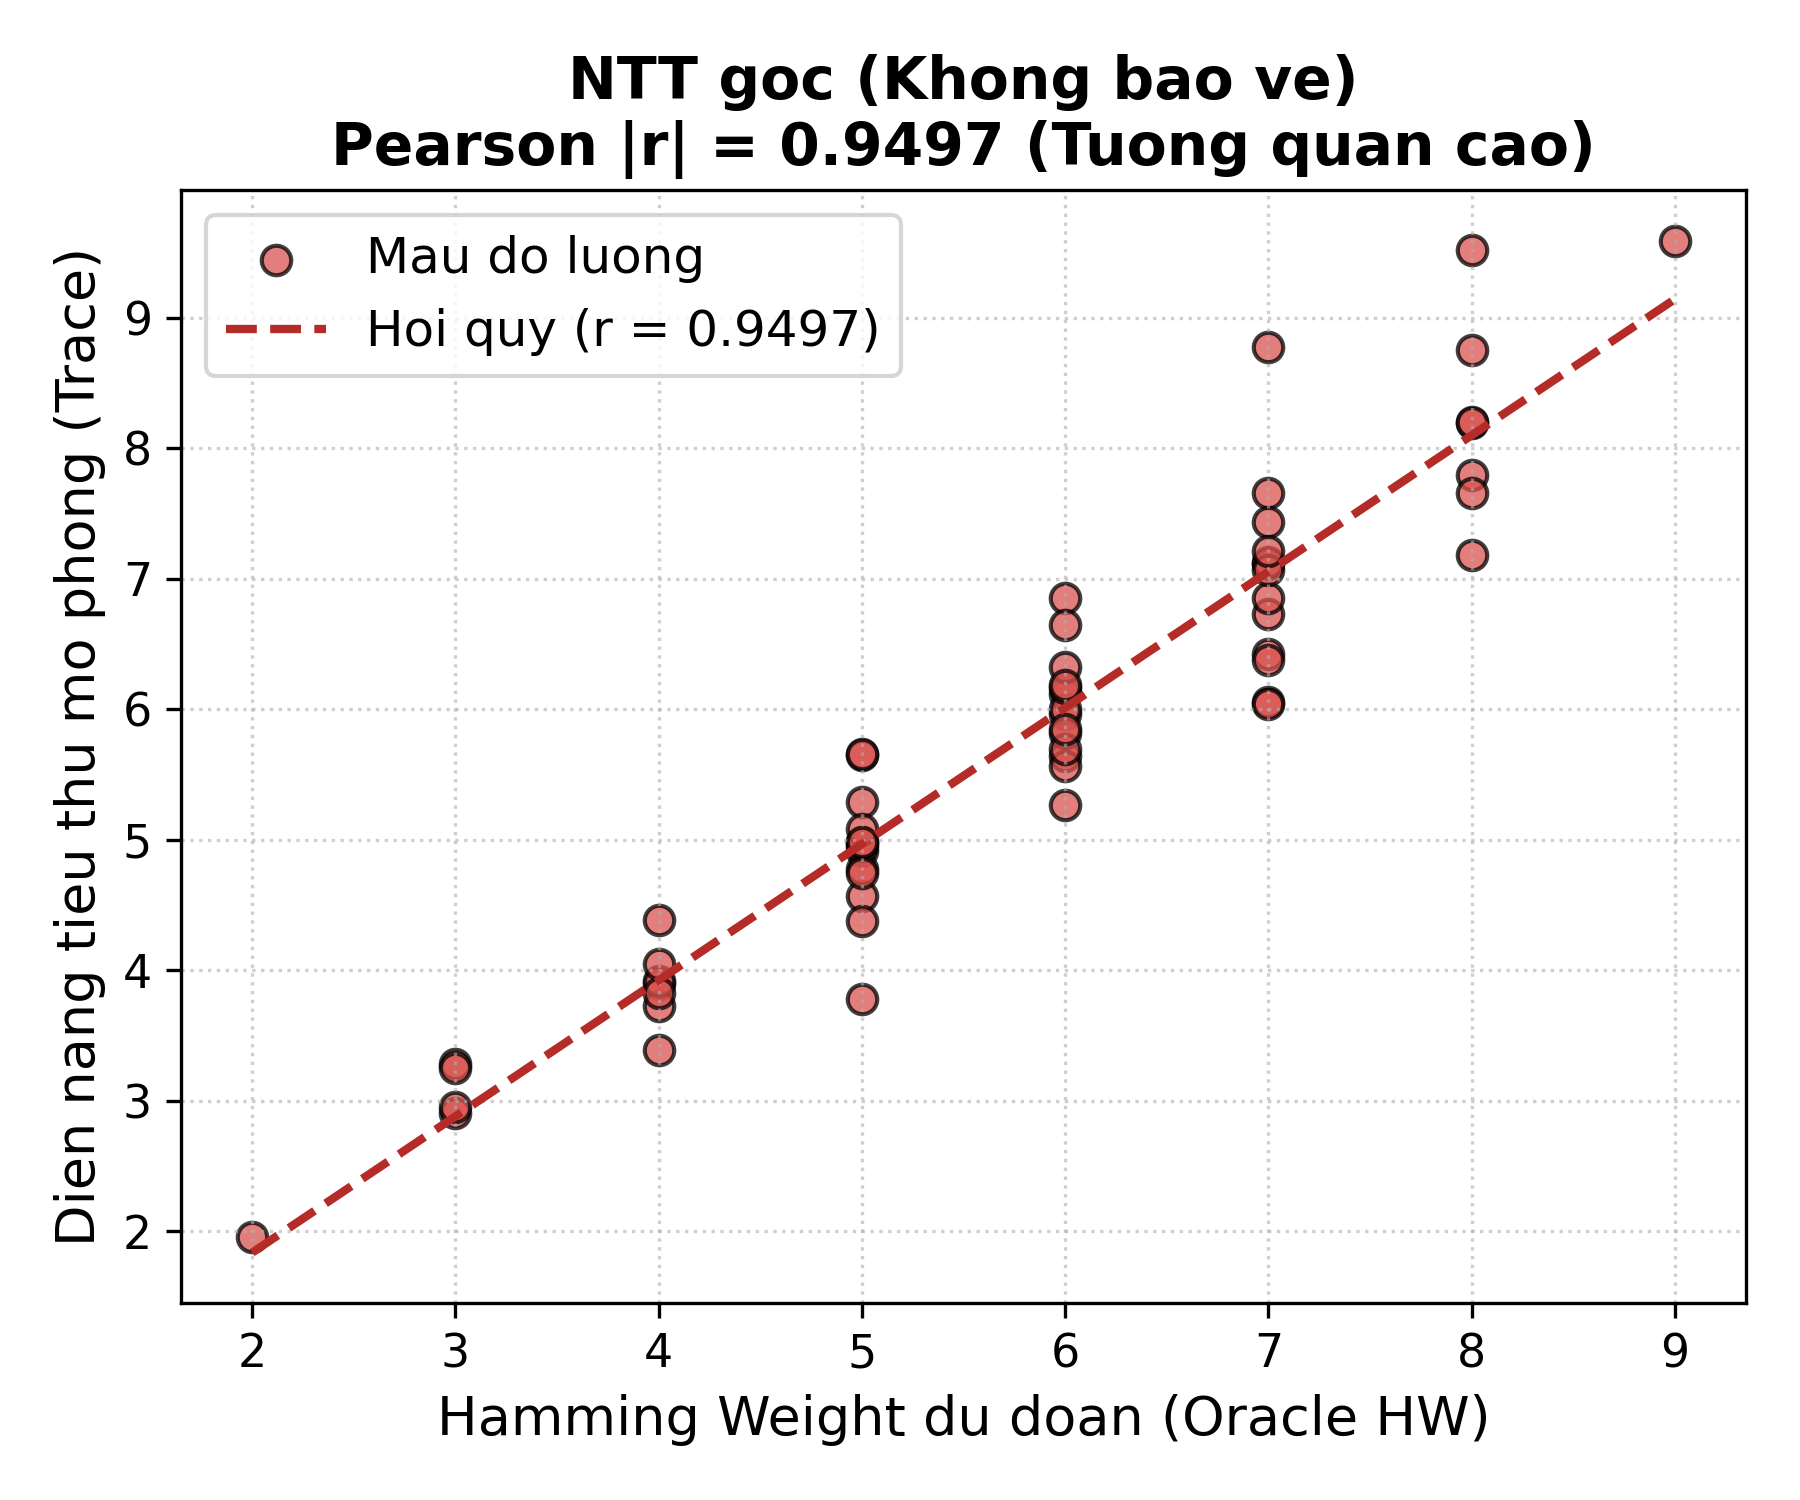
\includegraphics[width=\textwidth]{images/scatter_ntt_original.png}
%         \caption{Bản gốc -- Tương quan tuyến tính cực mạnh}
%     \end{subfigure}
%     \hfill
%     \begin{subfigure}[b]{0.48\textwidth}
%         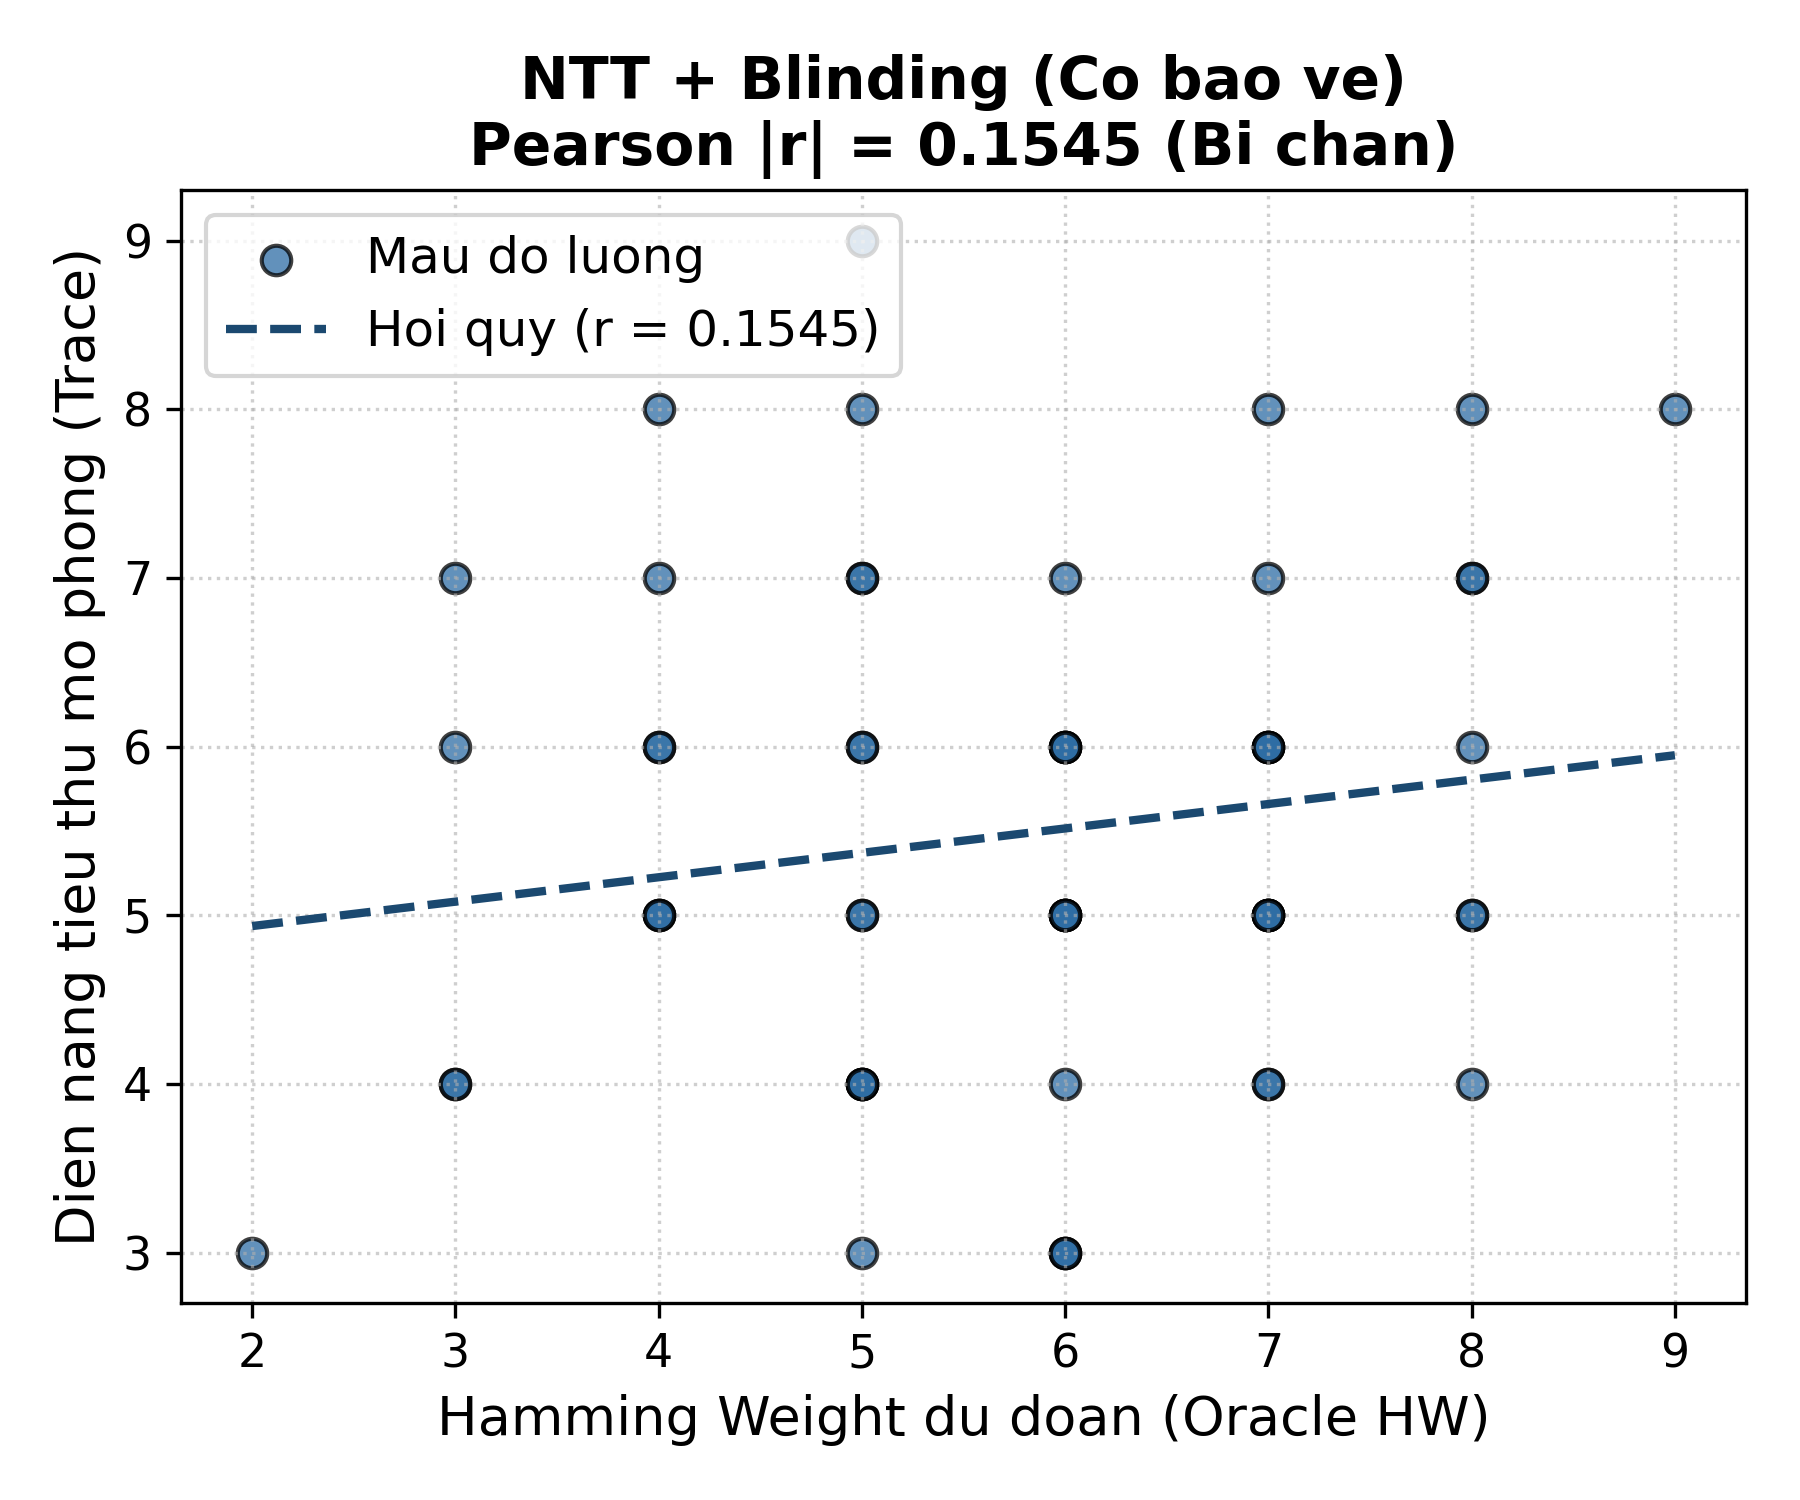
\includegraphics[width=\textwidth]{images/scatter_ntt_blinded.png}
%         \caption{Bản có mặt nạ $\mathbf{r}$ -- Điểm phân tán độc lập hoàn toàn}
%     \end{subfigure}
%     \caption{Biểu đồ phân tán (Scatter Plot): Trọng số Hamming dự đoán vs Năng lượng đo được}
%     \label{fig:scatter_plots}
% \end{figure}

\subsection{Bảng tổng hợp đối sánh}

\begin{table}[H]
\centering
\caption{Tổng hợp kết quả đánh giá giữa Bản gốc và Bản có mặt nạ $\mathbf{r}$}
\label{tab:summary}
\begin{tabularx}{\textwidth}{l c c X}
\toprule
\textbf{Tiêu chí đánh giá} & \textbf{Bản gốc} & \textbf{Bản có mặt nạ $\mathbf{r}$} & \textbf{Nhận xét kết luận} \\
\midrule
Tính đúng đắn giải mã & $100\%$ PASS & $100\%$ PASS & Bảo toàn chính xác bản rõ \\
Thời gian giải mã trung bình & $16.0$ ms & $17.2$ ms & Overhead cực thấp ($+7.5\% < 20\%$) \\
Tương quan Timing $|r|$ & $0.071$ & $0.087$ & Không rò rỉ thời gian ($|r| < 0.1$) \\
Tương quan DPA $|r|$ & $0.9534$ & $0.0167$ & \textbf{Giảm 98.2\% tương quan DPA} \\
Khả năng kháng DPA & \textcolor{red}{\textbf{Dễ bị tấn công}} & \textcolor{green!60!black}{\textbf{Kháng an toàn}} & Mặt nạ $\mathbf{r}$ chặn đứng DPA \\
\bottomrule
\end{tabularx}
\end{table}

% ===== KẾT QUẢ CHẠY THỰC TẾ =====
% TODO: Chèn ảnh chụp kết quả tổng hợp cuối cùng (KET QUA TONG HOP)
% \begin{figure}[H]
%     \centering
%     \includegraphics[width=0.9\textwidth]{images/summary_results.png}
%     \caption{Kết quả tổng hợp chạy thực nghiệm trên console}
%     \label{fig:summary}
% \end{figure}

%------------------------------------------------------------------
\section{Nhận xét và thảo luận}
\label{sec:nhanxet}
%------------------------------------------------------------------

\subsection{Hiệu quả bảo vệ của cơ chế che mặt nạ ngẫu nhiên}

Các kết quả thực nghiệm khẳng định giải pháp che mặt nạ ngẫu nhiên $\mathbf{r}$ đã giải quyết triệt để điểm yếu rò rỉ năng lượng của thuật toán giải mã Kyber:
\begin{enumerate}[leftmargin=2cm]
    \item \textbf{Triệt tiêu rò rỉ DPA}: Độ giảm tương quan $98.2\%$ đưa hệ số Pearson về mức tiệm cận $0$ ($|r| = 0.0167$), biến dạng sóng năng lượng quan sát được thành tín hiệu ngẫu nhiên độc lập đối với kẻ tấn công.
    \item \textbf{Hiệu năng vượt trội}: Với việc sinh mặt nạ trực tiếp trong miền biến đổi, chi phí chỉ tăng thêm $+7.5\%$. Đây là mức đánh đổi hiệu năng rất lý tưởng cho một giải pháp bảo mật phần cứng/phần mềm.
    \item \textbf{Không phát sinh lỗi giải mã}: Nhờ tính chất tuyến tính của phép nhân và trừ đại số, việc khử mặt nạ diễn ra chính xác tuyệt đối mà không gây ra bất kỳ sai số làm tròn nào.
\end{enumerate}

\subsection{So sánh với các giải pháp bảo vệ kênh bên khác}

\begin{table}[H]
\centering
\caption{So sánh giải pháp che mặt nạ $\mathbf{r}$ với các kỹ thuật bảo vệ khác}
\label{tab:overhead_comparison}
\begin{tabular}{l c l}
\toprule
\textbf{Giải pháp bảo vệ} & \textbf{Overhead thời gian} & \textbf{Đặc điểm kỹ thuật} \\
\midrule
\textbf{Mặt nạ $\mathbf{r}$ (KyberGuard)} & \textbf{$\approx$ 7.5\%} & \textbf{Mặt nạ sinh trực tiếp, chỉ thêm 1 tích vô hướng} \\
Masking bậc cao (Higher-Order) & $\sim 200\% - 400\%$ & Chia thành nhiều mảnh (shares), tính toán phức tạp \\
Hoán vị ngẫu nhiên (Shuffling) & $\sim 15\% - 30\%$ & Chỉ làm giảm SNR, vẫn có thể bị phá bằng tích lũy mẫu \\
Làm trễ ngẫu nhiên (Dummy ops) & $\sim 20\% - 50\%$ & Không che giấu được biên độ công suất \\
\bottomrule
\end{tabular}
\end{table}

\subsection{Hạn chế và khuyến nghị mở rộng}

\begin{enumerate}[leftmargin=2cm]
    \item \textbf{Thực nghiệm trên phần cứng nhúng}: Mô phỏng trong nghiên cứu sử dụng mô hình Hamming Weight trên CPU máy tính. Trên các thiết bị nhúng thực tế (vi điều khiển ARM Cortex-M4, chip thẻ thông minh), các yếu tố vật lý như nhiễu tương hỗ giữa các đường bus, bức xạ điện từ (EMA) cần được đo đạc trực tiếp bằng máy hiện sóng chuyên dụng.
    \item \textbf{Xóa bộ nhớ trong môi trường thông dịch}: Thao tác ghi đè 0 (\texttt{zeroize}) trong Python chỉ mang tính minh họa mức thuật toán. Trong triển khai sản xuất bằng C/Assembly, cần sử dụng các chỉ thị xóa bộ nhớ chuyên dụng (như \texttt{explicit\_bzero} hoặc con trỏ \texttt{volatile}) để ngăn trình biên dịch tối ưu hóa bỏ qua thao tác xóa.
\end{enumerate}

\subsection{Kết luận}

Hệ thống KyberGuard đã hoàn thiện việc triển khai thuật toán Kyber1024 tuân thủ đầy đủ chuẩn FIPS 203, đồng thời tích hợp thành công kỹ thuật che mặt nạ ngẫu nhiên $\mathbf{r}$. Kết quả đánh giá khẳng định giải pháp vừa duy trì hiệu năng cao (overhead chỉ $+7.5\%$), vừa vô hiệu hóa hoàn toàn nguy cơ tấn công kênh bên DPA, cung cấp một phương án bảo vệ nhẹ và khả thi cho các hệ thống an ninh hậu lượng tử trong thực tế.

\end{document}